\subsection{ROLLO: Reactor evOLutionary aLgorithm Optimizer}
\begin{frame}
    \frametitle{ROLLO: Reactor evOLutionary aLgorithm Optimizer}
    \begin{figure}
        
\includegraphics[width=0.7\linewidth]{figures/rollo-logo.png} 
        \caption{ROLLO (Reactor evOLutionary aLgorithm Optimizer) logo.}
    \end{figure}
    \begin{itemize}
        \item ROLLO (Reactor evOLutionary aLgorithm Optimizer) is a Python package 
        that applies evolutionary algorithms to optimize nuclear reactor design
        \item ROLLO provides a general genetic algorithm framework, sets up 
        parallelization for the user, and promotes usability with an input file that
        only exposes mandatory parameters
        \item Designed to be: effective, flexible, open-source, parallel, reproducible
    \end{itemize}
\end{frame}

\begin{frame}
    \frametitle{How does ROLLO work?}
    \begin{minipage}[c]{0.45\textwidth}
        \begin{itemize}
            \item Reads and validates the JSON input file
            \item Initializes the \acrfull{DEAP} genetic algorithm hyperparameters
            \item Runs the genetic algorithm  
            \item During the run, nuclear modeling software evaluates each individual 
            reactor model's fitness
        \end{itemize}
    \end{minipage}\hfill
    \begin{minipage}[c]{0.52\textwidth}
        \centering
        \begin{figure}
            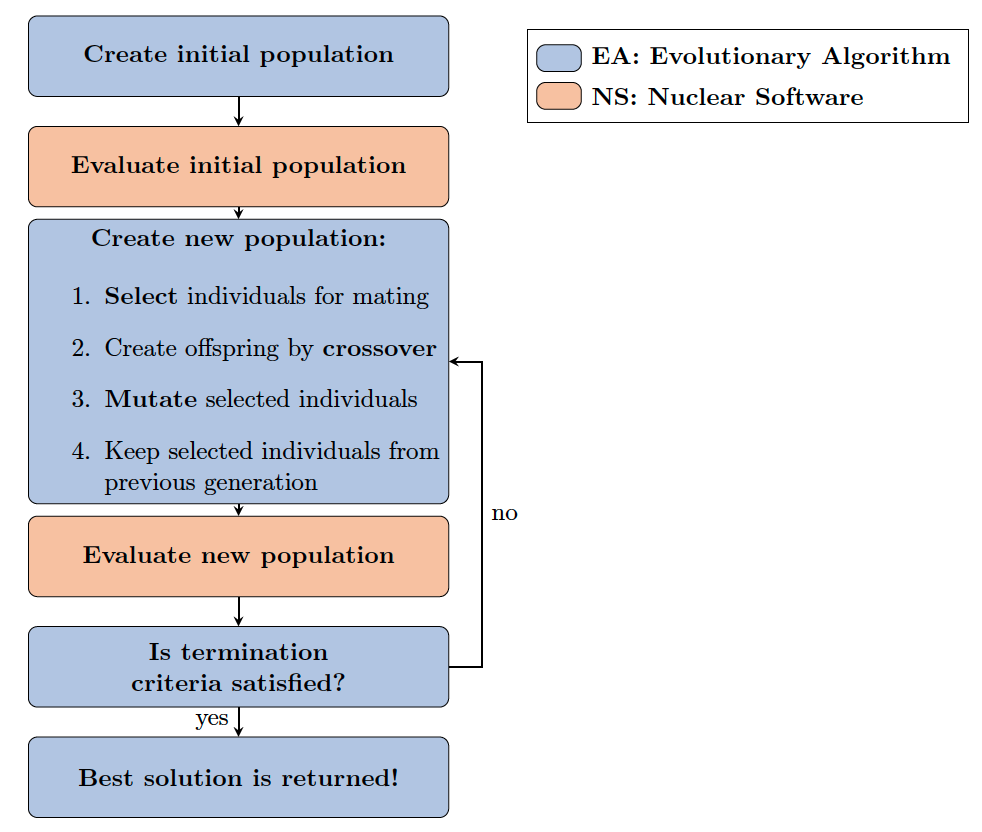
\includegraphics[width=\linewidth]{figures/rollo-flow.png} 
            \caption{ROLLO Genetic Algorithm Flow.}
        \end{figure}
    \end{minipage}

    For each ROLLO optimization simulation, one must \textbf{balance convergence and 
    computational cost}. 

    ROLLO's purpose is to help the human reactor designer narrow down reactor design 
    search space. The reactor designer uses the \textbf{computational power 
    available}, to \textbf{narrow down the search space} as much as possible.
\end{frame}
